\section{The Human Skin}\label{sec:chp1sec1}
Skin is the largest organ of the human body and consists of three main layers; epidermis, dermis and subcutaneous fat  \cite{anderson1981optics} (see Fig.\ref{fig:SkinAnatomy}).\\
		\begin{figure}
		\centering
		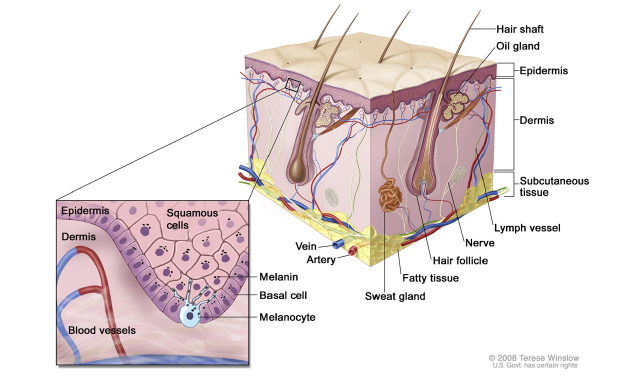
\includegraphics[width = 0.8\textwidth]{Chapter1/Figuers/SkinAnatomy.png}	
	\caption[Skin Anatomy]{Anatomy of the skin, showing the three structure layers of epidermis, dermis and subcutaneous tissue \cite{korotkov2012computerized}.}
		\label{fig:SkinAnatomy}
		\end{figure}	 
\begin{description}
	\item[Epidermis] is the outer layer or surface of the skin. This layer is divided into four sub-layers from top to bottom; stratum corneum, stratum granulosum, stratum spinosum and stratum basal \cite{mcgrath2010anatomy}.

The aforementioned layers contain four types of cells including keratinocytes, melanocytes, Langerhans' cells and Merkel cells. 
The majority of the cells in the epidermis are keratinocytes, the main force for continuous renewal of the skin \cite{mcgrath2010anatomy}.
These cells contain two main attributes of division and differentiation which enable them to renew the outer layer of the epidermis within thirty days.
During this journey, the keratinocytes, which are produced by division of the basal cells (keratinocytes in the basal layer are called basal cells), will move to the next layer while they go through a differentiation process.
Differentiation refers to this morphology and biochemistry transformation of the cells.
At the end of this journey, the keratinocyte cells will lose their nuclie and be transformed to flattened cells filled with keratine.
These cells form the outer most layer of the epidermis (stratum corneum).
At the end of the differentiation process, the corneocytes lose their cohension and separate from the surface in the desquamation process, resulting in renewed skin.

Langerhans' cells are responsible for the detection of foreign bodies (antigens) which invade the epidermis, transporting them to the local lymph nodes, while Merkel cells act as mechanosensory receptors in response to touch, forming close connections with sensory nerve endings \cite{mcgrath2010anatomy}.

Melanocyte cells are found in the basal layer of the epidermis \cite{mcgrath2010anatomy}.
These cells are responsible for distributing packages of melanin pigment, which lead to individual skin and hair colors, to the surrounding keratinocytes.
This chromophore mainly protects the subcutaneous tissue from being damaged by UV radiation.
Whenever the level of UV radiation increases, melanocytes start producing more melanin, resulting in our tanning reaction to sun exposure.
Melanin is the major chromophore of the epidermis which occupies the top 50-100 \si{\micro\meter}, with the exception of superior layers of epidermis.  

In most light propagation models through skin, the sublayers of epidermis are considered as one layer~\cite{lu2000modeling,jolivot2011developpement}.
The epidermal thickness can vary depending on different body parts, however on average, it is usually around 0.1 mm.
The most external sublayer of the epidermis is the stratum corneum.
It is composed of dry dead cells without organelles and is filled with keratin fibres.
Light is absorbed mainly in this layer, due to the epidermis major component melanin.	

\item[Dermis] is the middle layer between the epidermis and the hypodermic layer.
This layer is thicker than the epidermis, with an average thickness of 0.6 to 3 mm \cite{anderson1981optics}. 
The thermoregulation, the mechanical resistance and nourishing of the epidermis are the main functions of this layer. 
The dermis is composed of elastic collagen fibres, blood vessels, nerves, lymph vessels, hair follicles and sweat glands but its principal molecules, with relevant optical properties, are haemoglobin, carotene and bilirubin. 
Haemoglobin is a chromophore of red colour found in the microvascular network of the dermis, typically 100-500 \si{\micro\meter} below the skin's surface. 
This chromophore carries oxygen through vessels and capillaries and accordingly is called oxy-haemoglobin since it contains oxygen and deoxy-haemoglobin. 
The dermis is divided into two sublayers, the papillary dermis with the principal function of thermoregulation and the reticular dermis which gives the skin its strength and elasticity. 

\item[Subcutaneous fat] or hypodermic fat is the deepest layer of the skin, with an average thickness of 4 to 9 mm. 
This layer is composed of connective tissues, fat cells and blood vessels. 

\end{description}

	
% Nevertheless, it is not the aesthetic results of melanocyte activity that draw our attention, but their malignant transformation potential. Although cancer can develop in almost any cell in the body, certain cells are more cancer-prone than others and the skin is no exception. Most skin cancers develop from non-pigmented basal and squamous keratinocytes. Their transformation results in basal cell carcinoma and squamous cell carcinoma, respectively [1, 4]. However, melanocytes that undergo a malignant transformation produce a less common but far more deadly and aggressive cancer: malignant melanoma. The epidemiology and treatment of this cancer, as well as some skin lesions known as its precursors, are described in the following sections.



Cancer can develop in almost any cell in the body. 
However, certain cells are more cancer prone compared to others and the skin is no exception. 
The three most common malignant skin cancers are called basal cell carcinoma, squamous cell carcinoma and melanoma which develop from basal cells, squamous keratinocytes, and melanocytes, respectively. 
Melanocyte cells and their transformation, due to their malignant transformation potential, are our main concern in this thesis. 
Melanoma is less common in comparison to basal cell carcinoma and squamous cell carcinoma.
However, it is the deadliest and most aggressive type of skin cancer. 
The characteristics and treatment of this cancer, as well as some skin lesions very prone to malignancy are described in the following sections.


  %%% Local Variables: 
  %%% mode: latex
  %%% TeX-master: "../thesis"
  %%% End: 